\documentclass{article}
\usepackage{graphicx}
\usepackage{float}
\usepackage{amsmath}
\usepackage{lastpage}
\usepackage[margin=0.85in]{geometry}
\usepackage{fancyhdr}
\pagestyle{fancy}
\lhead{CSC373 Summer 2015}
\chead{Tutorial 7}
\rhead{TA: Eric Zhu}
\cfoot{Page \thepage~of~\pageref{LastPage}}
%\setlength{\parindent}{0pt}
\begin{document}

In this tutorial let's look at the vertex-cover problem 
\footnote{Based on 35.1 and 35.4 of {\it Introduction to Algorithms
2nd Edition} by Cormen, Leiserson, Rivest, and Stein.}. 
A {\bf vertex cover} is essentially a subset of vertexes that covers all the 
edges in the graph.
Formally, given an undirected graph $G = (V, E)$, a vertex cover is a subset
$V' \subseteq V$ such that if $(i, j)$ is an edge of $G$, then either
$i \in V'$ or $j \in V'$ (or both).

The {\bf vertex cover problem}, on the other hand, is to to find the vertex
cover with the minimum number of vertexes - the {\bf optimal vertex cover}.
It looks like we can formulate the problem as Linear Programming problem.
So let's work out the formulation first.
\begin{figure}[H]
\centering
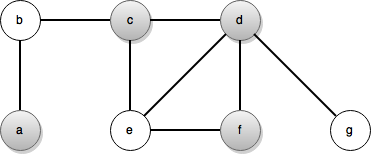
\includegraphics[width=0.35\textwidth]{vertexcover1.png}
\caption{An example solution to VERTEX-COVER.}
\end{figure}

First let's consider what to use as the decision variables.
Imagine you create an vector $X$ of the size equals to the number of vertexes, 
$|V|$, in the graph $G$. 
Then you map each position $X_i$ in the vector uniquely to a vertexes $V_i$.
If a vertex is used, mark a 1 at its position in the vector. If a vertex
is not used, mark a 0.
This way, a subset of $V$ can be represented as an $X$ vector with 1s at
positions corresponding to the selected vertexes, and 0s for the skipped
vertexes.

Now, let's come up with the objective function, which we are trying to optimize.
We already know that the vertex cover problem is to find the cover with
the minimum number of vertexes. A cover is a subset, and we want the size
of the subset to be minimum. Thus, the objective function is simply the
number of vertexes selected. We can express this value using our vector $X$.
Since 1s in $X$ correspond to the vertexes selected and 0s correspond to the
vertexes skipped, the sum of all elements in the vector $X$ is equal to the
objective function: $\sum_{i \in V} X_i$.

If we only have the above, the optimal solution is going to be $X$ with 0s at
all the positions, as it minimizes the objective function.
However, the vertex cover problem requires the selected subset of vertexes to
cover all the edges in the graph. This means a set of constraints to our
possible solutions. Now let's translate the requirement into constraints:
\begin{itemize}
\item Any edge consists of two vertexes, let's use $(i,j)$
	to denote an edge that connects vertexes $i$ and $j$.
\item If both $i$ and $j$ are selected as part of the vertex cover,
	then $X_i + X_j = 2$, because $X_i = 1$ and $X_j = 1$, and the edge
	$(i,j)$ is covered.
\item If either $i$ or $j$ is selected, then $X_i + X_j = 1$, because only one 
	equals 1, and the edge $(i,j)$ is covered.
\item If neither $i$ nor $j$ is selected, then the edge $(i,j)$ is not covered,
	which cannot be the case since the vertex cover must cover all edges.
\item Thus, for any edge $(i, j) \in E$, $X_i + X_j \ge 1$.
\end{itemize}

Now we have a constraint for every edge in the graph, and we can complete our
formulation:
\begin{equation}
\label{eq:vc_ilp}
\begin{split}
	\min \sum_{i \in V} X_i\\
	X_i + X_j \ge 1, \forall (i, j) \in E\\
	X_i \in \{0, 1\} \forall i \in V
\end{split}
\end{equation}

Actually, this formulation is not a Linear Programming problem, rather, it is
a classic example of Integer Linear Programming problem, because of the integer
constraints on the decision variables.
In general, Integer Linear Programming problems are not polynomial-time
solvable. (Why?) However, for {\bf vertex cover problem}, we can use Linear
Programming to find an approximation of the optimal vertex cover, within 2 times
the size of the optimal cover: 
we replace the integer constraints $X_i \in \{0,1\}$
with $X_i \in [0, 1]$ so that $X_i$ can take on real numbers.
In fact, we can simplify a bit more and use $X_i \ge 0$, since the objective
function is already trying to minimize the value of $X_i$.
Now we have a Linear Programming formulation:
\begin{equation}
\label{eq:vc_lp}
\begin{split}
	\min \sum_{i \in V} X_i\\
	X_i + X_j \ge 1, \forall (i, j) \in E\\
	X_i \ge 0 \forall i \in V
\end{split}
\end{equation}
We can plug-in the Simplex Algorithm and solve the above problem, but the
solution we get will be real numbers. So we need to round the $X_i$s.
Let the rounded result be $X_i'$:
\begin{equation}
\label{eq:vc_rounding}
	X_i' = \left\{\begin{matrix}
		1, & if~X_i \ge \frac{1}{2}\\ 
		0, & if~X_i < \frac{1}{2}
	\end{matrix}\right., 
	\forall i \in V
\end{equation}
Finally, we output the vector $X'$ as our approximate optimal vertex cover.

How do we know this rounded solution is even a vertex cover? Consider any edge 
$(i,j) \in E$. By the constraints in Equation \ref{eq:vc_lp}, we know that
$X_i + X_j \ge 1$, which implies that at least one of $X_i'$ and $X_j'$ is
at least 1/2. Therefore, at least one of $i$ and $j$ will be included in the
vertex cover based on the rounding rule in Equation \ref{eq:vc_rounding}, 
and so every edge will be covered, and $X'$ is a vertex cover.

Next, how do we know the size of vertex cover $X'$ is within 2 times the size
of the optimal vertex cover?
Let the optimal solution to the original Integer Linear Programming
problem (Equation \ref{eq:vc_ilp}) be $X^{*}$.
It turns out $X^{*}$ is also a feasible solution to the Linear Programming
problem (Equation \ref{eq:vc_lp}), since the integer constraints are
more restrict then the non-negativity constraints. Since $X$ is the optimal
solution to the Linear Programming problem, the value of the objective function
given $X$ should be smaller than that given $X^{*}$, that is:
\begin{equation}
\sum_{i \in V} X_{i} \le \sum_{i \in V} X_{i}^{*}
\end{equation}
Because of the rounding, we have the following relationship between the 
real number solution $X$ and the rounded integer solution $X'$:
\begin{equation}
	\begin{split}
		\sum_{i \in V} X_{i} 
		&\ge \sum_{i \in V:X_i \ge 1/2} X_i\\
		&\ge \sum_{i \in V:X_i \ge 1/2} \frac{1}{2}\\
		&= \sum_{i \in V} X_i'\cdot \frac{1}{2}
	\end{split}
\end{equation}
Combining the above equations, we have the relationship between $X'$ and $X^{*}$:
\begin{equation}
\sum_{i \in V} X_i'\cdot \frac{1}{2} 
\le \sum_{i \in V} X_{i} \le \sum_{i \in V} X_{i}^{*}
\end{equation}

\end{document}
